\begin{figure}
 \centering
 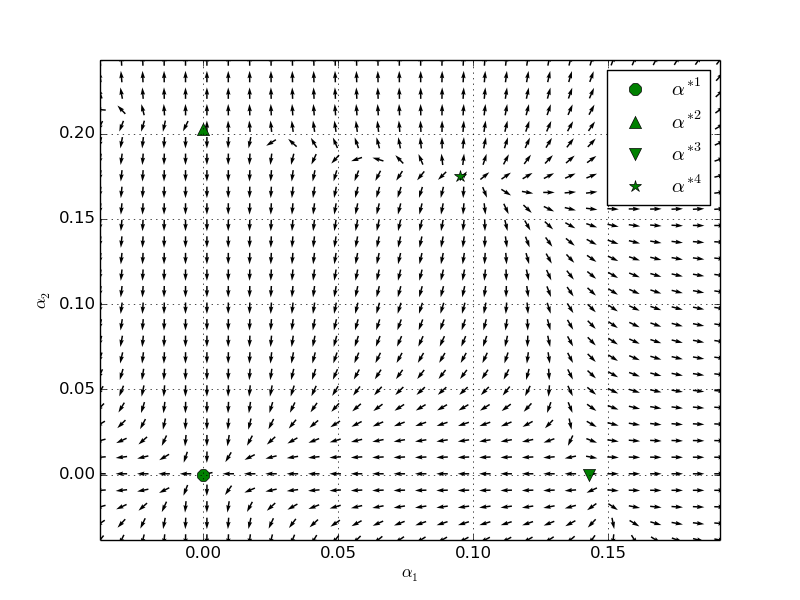
\includegraphics[scale=0.7]{Python/plots/RG_flow/RG_flow3_3_6_0_5_2_3_0.png}
 \caption{Ein Phasenraumdiagramm mit wechselwirkendem IR-Fixpunkt. Die Parameter
 sind $(\Nc,\Nd,\nfc,\nsc,\nfd,\nsd,\nfj,\nsj)=(3,3,6,0,5,2,3,0)$. In \cite{Scale_of_dark_QCD} 
 wurde für diese Parameter die Entkopplungsskala $Q=518\,\text{GeV}$ berechnet.}
 \label{fig:messbarkeit:IR-Fix}
\end{figure}
